\documentclass[12pt,a4paper]{article}
\usepackage{fontspec}
\setmainfont{Times New Roman}
\setsansfont{Arial}
\setmonofont{Courier New}
\usepackage[provide=*,english,romanian]{babel}
\usepackage{amsmath,amssymb,graphicx,geometry,setspace}
\usepackage{fancyhdr,caption,float,listings,xcolor,booktabs,longtable,array,calc}
\usepackage{subcaption,etoolbox,upquote}
\usepackage[unicode,hidelinks]{hyperref}
\geometry{top=2cm,bottom=2cm,left=2.5cm,right=2.5cm}
\setstretch{1.5}
\setlength{\parindent}{0pt}
\setlength{\parskip}{5pt}
\makeatletter
\renewcommand\section{\@startsection{section}{1}{0pt}{16pt}{7pt}{\normalfont\Large\bfseries}}
\renewcommand\subsection{\@startsection{subsection}{2}{0pt}{12pt}{5pt}{\normalfont\large\bfseries}}
\renewcommand\subsubsection{\@startsection{subsubsection}{3}{0pt}{9pt}{4pt}{\normalfont\normalsize\bfseries}}
\makeatother
\setcounter{secnumdepth}{-1}
\pagestyle{fancy}
\fancyhf{}
\rfoot{\thepage}
\renewcommand{\headrulewidth}{0pt}
\setlength{\headheight}{15pt}
\captionsetup{font=small,labelfont=bf,skip=6pt,justification=raggedright,singlelinecheck=false}
\captionsetup[figure]{position=above}
\lstset{language=C,basicstyle=\ttfamily\fontsize{9.5}{11.5}\selectfont,
  columns=fullflexible,showstringspaces=false,tabsize=2,numbersep=8pt,
  frame=single,rulecolor=\color{black!35},breaklines=true,keepspaces=true,
  xleftmargin=4pt,xrightmargin=4pt,aboveskip=8pt,belowskip=8pt}
\AtBeginEnvironment{lstlisting}{\singlespacing}
\AtBeginEnvironment{longtable}{\small\singlespacing}
\setlength{\emergencystretch}{3em}
\providecommand{\tightlist}{\setlength{\itemsep}{0pt}\setlength{\parskip}{0pt}}
\providecommand{\passthrough}[1]{#1}
\providecommand{\pandocbounded}[1]{#1}
\hypersetup{pdftitle={Sisteme de operare — Laborator 7 și 8},pdfauthor={Tacu Igor}}
\clubpenalty=10000
\widowpenalty=10000
\displaywidowpenalty=10000
\begin{document}
\begin{titlepage}
\thispagestyle{empty}
\begin{center}
\setstretch{1.18}

\includegraphics[width=0.23\textwidth]{scripts/report-style/utm-logo.png}\\[12pt]
\textbf{MINISTERUL EDUCAȚIEI ȘI CERCETĂRII}\\
\textbf{AL REPUBLICII MOLDOVA}\\[4pt]
\textbf{Universitatea Tehnică a Moldovei}\\
\textbf{Facultatea de Calculatoare, Informatică și Microelectronică}\\
\textbf{Departamentul Inginerie Software și Automatică}\\[36pt]
{\fontsize{22}{26}\selectfont\textbf{Raport}}\\[10pt]
Lucrare de laborator nr. 7 și 8\\[8pt]
\textbf{\large Sisteme de operare}\\[24pt]
\textbf{Tema:} Procese, execuție de programe, redirecționare și comunicare prin pipe-uri
\end{center}
\vfill
\begin{flushright}
\setstretch{1.25}
Realizat de:\\
stud. gr. FAF-242, Tacu Igor\\[24pt]
Verificat de:\\
Reițman Patricia
\end{flushright}
\vfill
\begin{center}\textbf{Chișinău – 2026 }\end{center}
\end{titlepage}

\setcounter{page}{1}
\section{Scopul lucrării}\label{scopul-lucrux103rii}

Urmărirea ciclului de viață al proceselor și a descriptorilor moșteniți,
prin exemple Linux și programe xv6 de execuție și comunicare.

\section{Sarcina lucrării}\label{sarcina-lucrux103rii}

\begin{itemize}
\tightlist
\item
  Compilarea și executarea programelor run, zombie, redirect și pipeline
  pe Linux.
\item
  Observarea stării zombie, a codurilor de terminare și a efectului
  descriptorilor de pipe rămași deschiși.
\item
  Verificarea programelor run și pingpong în xv6, pe căi de succes și
  eroare.
\end{itemize}

\section{Considerații teoretice}\label{consideraux21bii-teoretice}

fork creează un proces copil, exec înlocuiește imaginea programului, iar
wait colectează starea de terminare. Un copil terminat rămâne zombie
până la colectare. Descriptorii sunt păstrați peste exec dacă nu sunt
configurați altfel, iar cititorul unui pipe vede EOF numai după
închiderea tuturor capetelor de scriere.

\section{Implementare. Rezultate
practice}\label{implementare.-rezultate-practice}

\subsection{Question and execution
environment}\label{question-and-execution-environment}

A shell pipeline and a child that replaces itself with another program
both depend on state that survives process creation or program
replacement. Lab 7 isolates that state under Linux: PIDs, wait status,
open descriptors, and pipe endpoints. Lab 8 applies the same ideas to
xv6, where the user API and kernel implementation are small enough to
inspect together. The revised experiments below were run in Ubuntu 24.04
x86\_64 over SSH and in QEMU with the committed xv6 source. The output
is from the new run, not the earlier SSH screenshots.

All six requested programs are present in this repository. Linux sources
are in {\ttfamily\fontsize{10}{12}\selectfont Lab7-8/linux}; xv6 sources
are {\ttfamily\fontsize{10}{12}\selectfont xv6/user/run\allowbreak{}.c}
and
{\ttfamily\fontsize{10}{12}\selectfont xv6/user/pin\allowbreak{}gpong.c}.
The complete xv6 tree includes the UPROGS registrations. Raw transcripts
are in
{\ttfamily\fontsize{10}{12}\selectfont Lab7-8/evide\allowbreak{}nce},
and the two runner scripts under
{\ttfamily\fontsize{10}{12}\selectfont scripts} retain the commands that
produced them.

\subsection{Lab 7 Replacing a child while preserving its
identity}\label{lab-7-replacing-a-child-while-preserving-its-identity}

{\ttfamily\fontsize{10}{12}\selectfont run.c} flushes the parent's
initial message before calling
{\ttfamily\fontsize{10}{12}\selectfont fork}. Otherwise buffered output
could be copied and later printed twice when stdout is redirected. The
child prints its identity, flushes that output, and invokes
{\ttfamily\fontsize{10}{12}\selectfont execvp} for an explicit command
or {\ttfamily\fontsize{10}{12}\selectfont execlp} for the default
{\ttfamily\fontsize{10}{12}\selectfont ls -l}. The parent waits for the
particular child PID with
{\ttfamily\fontsize{10}{12}\selectfont waitpid}, then distinguishes
normal exit from signal termination before interpreting the status bits.

The default listing, a UTC date command, and a deliberately absent
program exercise three paths. Both successful programs return status
zero. The absent executable returns from exec, prints the error, and
calls {\ttfamily\fontsize{10}{12}\selectfont \_exit(127)}. The parent
subsequently reports 127 for the child; the parent utility itself
returns normally after reporting that result. It would be misleading to
describe the parent's own exit code as 127 simply because that number
appears in its message.

\par\noindent\begin{minipage}{\linewidth}

\begin{lstlisting}
+ ./run
parent: my PID is 3310792
child: my PID is 3310793, my parent is 3310792
total 80
-rwxr-xr-x 1 root root 16528 Nov  9 14:21 pipeline
-rwxr-xr-x 1 root root 16400 Nov  9 14:21 redirect
-rwxr-xr-x 1 root root 16440 Nov  9 14:21 run
-rwxr-xr-x 1 root root 16440 Nov  9 14:21 zombie
parent: child 3310793 ended with status 0
+ ./run date -u +%Y-%m-%d
parent: my PID is 3310794
child: my PID is 3310795, my parent is 3310794
2026-11-09
parent: child 3310795 ended with status 0
+ ./run no_such_igor_program
parent: my PID is 3310796
child: my PID is 3310797, my parent is 3310796
exec: No such file or directory
parent: child 3310797 ended with status 127
\end{lstlisting}

\end{minipage}\par

Successful exec does not create an additional child and does not run the
fallback error branch. It replaces the calling child's address space
while retaining its PID and inherited descriptors. This is why the
listing appears between the child's identification and the parent's
completion message. The exact PID values are incidental; the
relationship between them is the part under test.

\subsection{Lab 7 Delaying collection of a terminated
child}\label{lab-7-delaying-collection-of-a-terminated-child}

{\ttfamily\fontsize{10}{12}\selectfont zombie.c} uses the same exec path
but makes the parent sleep before
{\ttfamily\fontsize{10}{12}\selectfont waitpid}. The child can finish
its listing while the parent is still alive. The process query selects
children of the saved background parent PID, which avoids mixing this
case with unrelated processes on the machine. The first query found a
{\ttfamily\fontsize{10}{12}\selectfont Z} entry for ls; after waiting
for the parent utility, the second query contained only the header.

\par\noindent\begin{minipage}{\linewidth}

\begin{lstlisting}
+ parent_pid=3310798
+ ./zombie
+ sleep 1
+ ps -o pid,ppid,stat,cmd --ppid 3310798
    PID    PPID STAT CMD
3310800 3310798 Z    [ls] <defunct>
+ wait 3310798
+ ps -o pid,ppid,stat,cmd --ppid 3310798
    PID    PPID STAT CMD
\end{lstlisting}

\end{minipage}\par

The zombie is not a program still executing the ls instructions. It is
the kernel's retained termination information awaiting collection. The
delay makes this normally short interval observable. Using
{\ttfamily\fontsize{10}{12}\selectfont \$!} immediately after launching
the parent and filtering with
{\ttfamily\fontsize{10}{12}\selectfont --ppid} ties the observed entry
to the experiment rather than to a coincidentally named process.

\subsection{Lab 7 Redirecting output by descriptor
reuse}\label{lab-7-redirecting-output-by-descriptor-reuse}

The redirection child closes descriptor 1 before opening
{\ttfamily\fontsize{10}{12}\selectfont out.txt}. Since open chooses the
lowest available descriptor, the new descriptor is 1. The later ls image
writes through the standard-output number it always uses, but that
number now refers to the file. The diagnostic is deliberately written to
stderr and remains visible outside the file. The parent waits and checks
the child's status before announcing completion.

The run reported
{\ttfamily\fontsize{10}{12}\selectfont open gave descriptor 1}; reading
the first lines of {\ttfamily\fontsize{10}{12}\selectfont out.txt}
displayed the saved listing. To redirect errors instead, close
descriptor 2 before opening the error file. The listing showed
{\ttfamily\fontsize{10}{12}\selectfont out.txt} as empty at the moment
ls inspected its metadata; ls was itself generating the bytes
subsequently read by head.

\subsection{Lab 7 A pipe whose reader needs every writer to
close}\label{lab-7-a-pipe-whose-reader-needs-every-writer-to-close}

{\ttfamily\fontsize{10}{12}\selectfont pipeline.c} creates one pipe and
two children. The ls child duplicates the write endpoint onto stdout.
The wc child duplicates the read endpoint onto stdin. Each child closes
both original endpoints after duplication, and the parent also closes
its copies before collecting both children. The ordinary program and
{\ttfamily\fontsize{10}{12}\selectfont ls /etc | wc -l} each returned
\textbf{215} in this environment. This is a measurement of the current
server's {\ttfamily\fontsize{10}{12}\selectfont /etc}, not a fixed
expected value for Ubuntu.

The revised program includes a bounded
{\ttfamily\fontsize{10}{12}\selectfont --delay-eof} mode. It retains the
parent's write endpoint for three seconds, then closes it. This
demonstrates the reader's dependence on the last writer without leaving
a permanently blocked process behind. The measured elapsed time was
about three seconds, and wc eventually returned the same count.

\par\noindent\begin{minipage}{\linewidth}

\begin{lstlisting}
+ ./pipeline
215
+ ls /etc
+ wc -l
215
+ ./pipeline --delay-eof
parent keeps the write end open for 3 seconds; wc waits for EOF
215

real    0m3.003s
user    0m0.001s
sys 0m0.006s
+ python3 /tmp/igor-os-review-20261109/scripts/check-broken-pipeline.py /tmp/igor-os-review-20261109
Part 4.3: pipeline is still running after two seconds
    PID    PPID STAT CMD
3310882 3310880 S    wc -l
Interrupted with SIGINT (Ctrl-C equivalent); return code -2
\end{lstlisting}

\end{minipage}\par

The handout's Part 4.3 was also executed literally: the parent's final
{\ttfamily\fontsize{10}{12}\selectfont close(p[1])} was omitted in a
test variant. After two seconds the parent was still running and ps
showed wc waiting. The test then interrupted the process group with
SIGINT, the terminal Ctrl-C signal. Its record is included in the block
above. The bounded delay mode is an additional experiment, not a
replacement for this broken case.

A pipe read can reach EOF only after buffered bytes have been consumed
and every descriptor referring to its write end has been closed. Copies
inherited through fork count too, which is why closing endpoints only in
the producer is insufficient.

\subsection{Lab 8 Reusing the lifecycle inside
xv6}\label{lab-8-reusing-the-lifecycle-inside-xv6}

The xv6 {\ttfamily\fontsize{10}{12}\selectfont run} utility defaults to
echo but also accepts a command and its arguments. This makes success
and failure reproducible without editing source between each test. It
calls fork, uses exec in the child, and waits in the parent.
{\ttfamily\fontsize{10}{12}\selectfont run} printed
{\ttfamily\fontsize{10}{12}\selectfont hello from the child} and status
zero; {\ttfamily\fontsize{10}{12}\selectfont run ls} listed the
generated filesystem;
{\ttfamily\fontsize{10}{12}\selectfont run no\_such\_igor\allowbreak{}\_program}
took the fallback branch and reported status one.

\par\noindent\begin{minipage}{\linewidth}

\begin{lstlisting}
$ run
parent: my pid is 87
child: my pid is 88
hello from the child
parent: child 88 ended with status 0
$ run no_such_igor_program
parent: my pid is 91
child: my pid is 92
exec failed
parent: child 92 ended with status 1
\end{lstlisting}

\end{minipage}\par

The Linux fallback uses 127 and the xv6 fallback uses 1 because those
values are explicitly chosen by the utilities. Exec failure does not
force every program or OS to choose the same status. The xv6 wait API
also differs from Linux waitpid: it collects a child and writes the
status through a pointer without selecting a particular PID in this
program.

\subsection{Lab 8 Passing a byte in each
direction}\label{lab-8-passing-a-byte-in-each-direction}

{\ttfamily\fontsize{10}{12}\selectfont pingpong.c} creates separate
parent-to-child and child-to-parent pipes before forking. The parent
sends one byte on the first pipe and blocks waiting on the second. The
child reads the byte, prints its ping message, and returns the byte on
the other pipe. Both processes close the endpoints they do not use; the
parent then waits to collect the child. The implementation checks every
one-byte read and write instead of assuming a transfer succeeded.

\par\noindent\begin{minipage}{\linewidth}

\begin{lstlisting}
$ pingpong
94: received ping
93: received pong
$
\end{lstlisting}

\end{minipage}\par

The observed ping-before-pong order follows from the data dependency.
Specifically,
{\ttfamily\fontsize{10}{12}\selectfont read(c2p[0], \&b, 1)} blocks the
parent until a reply byte is available; the later wait collects the
terminated child. Two pipes give each direction its own stream and make
ownership explicit.

\subsection{Interpretation and source
provenance}\label{interpretation-and-source-provenance}

These tests connect shell behavior to specific lifetime rules. Fork
copies descriptor references, exec preserves them, wait collects
termination state, and close can determine whether another process is
allowed to finish. The delayed EOF experiment is particularly useful
because its final count is unchanged while its completion time changes.
It distinguishes a communication-lifetime error from an incorrect
data-processing result.

The runner checks compilation with
{\ttfamily\fontsize{10}{12}\selectfont -Wall -Wextra -Werror}, verifies
the Linux cases, builds the complete xv6 image, and checks distinctive
output for run and pingpong. It does not claim that this limited set
proves arbitrary error recovery or all scheduling orders. MIT xv6
remains the upstream teaching system; the added utilities and their test
fixtures are identified in
{\ttfamily\fontsize{10}{12}\selectfont xv6/PROVENAN\allowbreak{}CE.md}
rather than presenting the entire kernel as newly authored code.

\subsection{Execution captures and code
excerpts}\label{execution-captures-and-code-excerpts}

All execution screenshots below are native Terminal captures supplied by
the author from direct Linux or xv6 execution. Linux tests use a
separate temporary directory containing sources and binaries; the xv6
capture includes an additional explicit echo command. PIDs and listing
contents identify these later screenshot runs. Earlier full transcripts
remain in the repository. Source excerpts are listed as selectable text,
and complete source files accompany the report.

\par

\medskip\noindent

\begin{minipage}{\linewidth}\setstretch{1.0}
\captionof*{figure}{Figura 1. Native Linux run execution}
\centering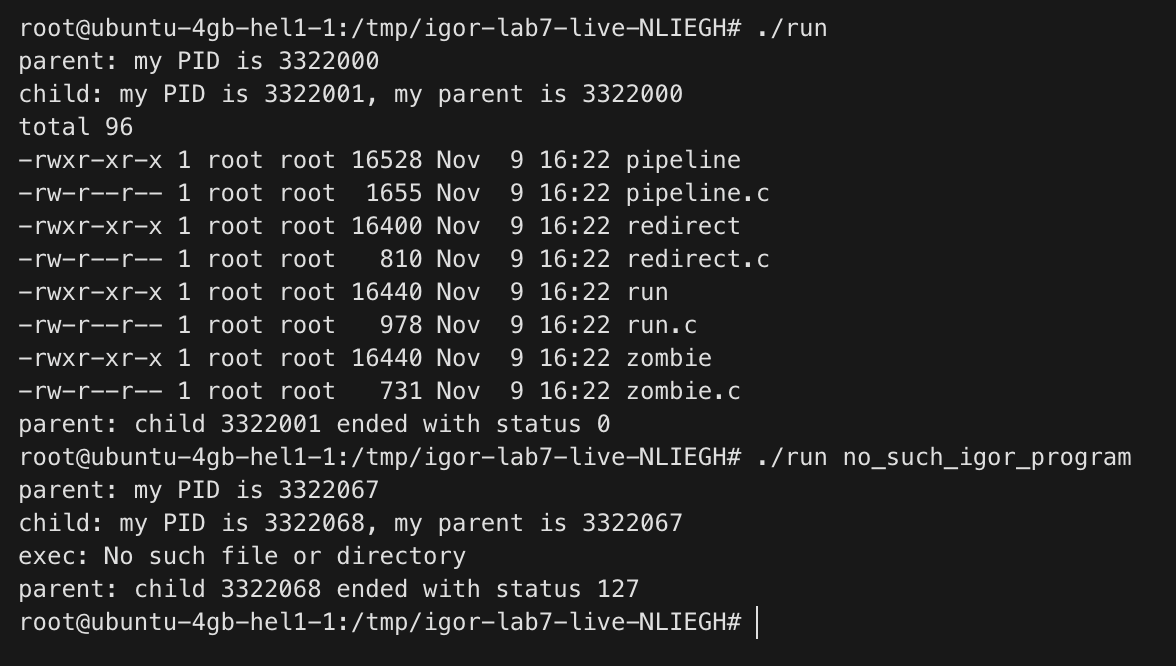
\includegraphics[width=\linewidth,height=0.67\textheight,keepaspectratio]{Lab7-8/evidence/screenshots/lab7-run-terminal.png}
\end{minipage}\par\medskip

\par

\medskip\noindent

\begin{minipage}{\linewidth}\setstretch{1.0}
\captionof*{figure}{Figura 2. Native Linux zombie state before and after collection}
\centering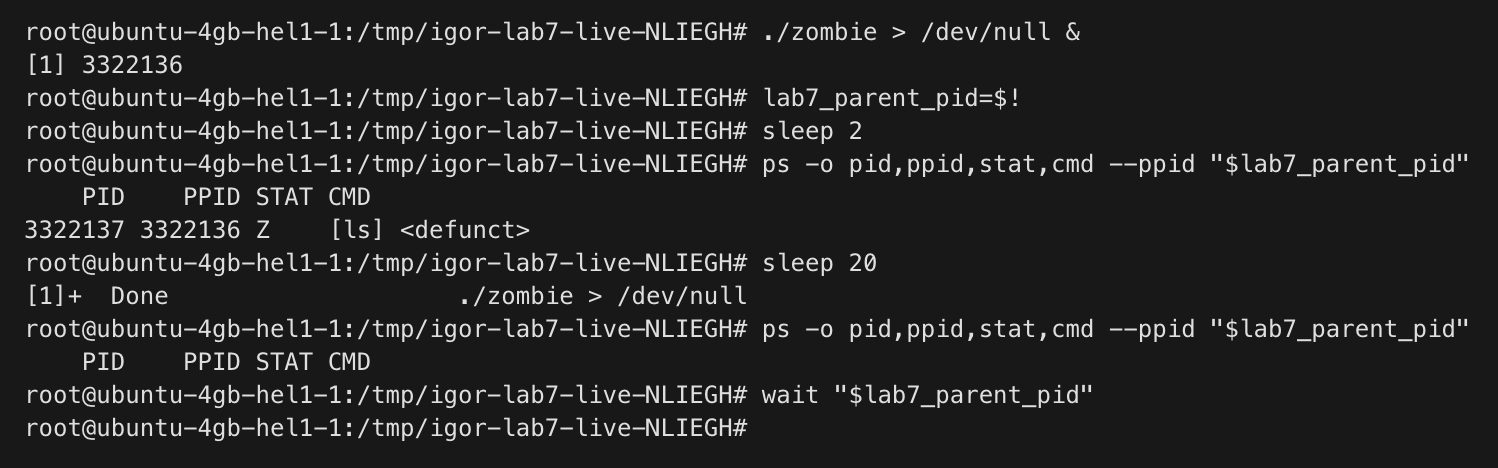
\includegraphics[width=\linewidth,height=0.67\textheight,keepaspectratio]{Lab7-8/evidence/screenshots/lab7-zombie-terminal.png}
\end{minipage}\par\medskip

\par

\medskip\noindent

\begin{minipage}{\linewidth}\setstretch{1.0}
\captionof*{figure}{Figura 3. Native Linux descriptor redirection and file output}
\centering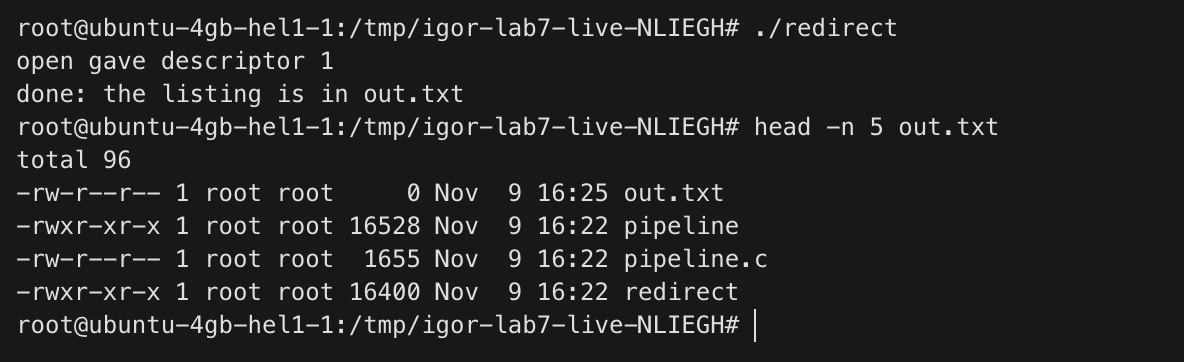
\includegraphics[width=\linewidth,height=0.67\textheight,keepaspectratio]{Lab7-8/evidence/screenshots/lab7-redirection-terminal.png}
\end{minipage}\par\medskip

\par

\medskip\noindent

\begin{minipage}{\linewidth}\setstretch{1.0}
\captionof*{figure}{Figura 4. Native Linux pipeline comparison and omitted-close experiment}
\centering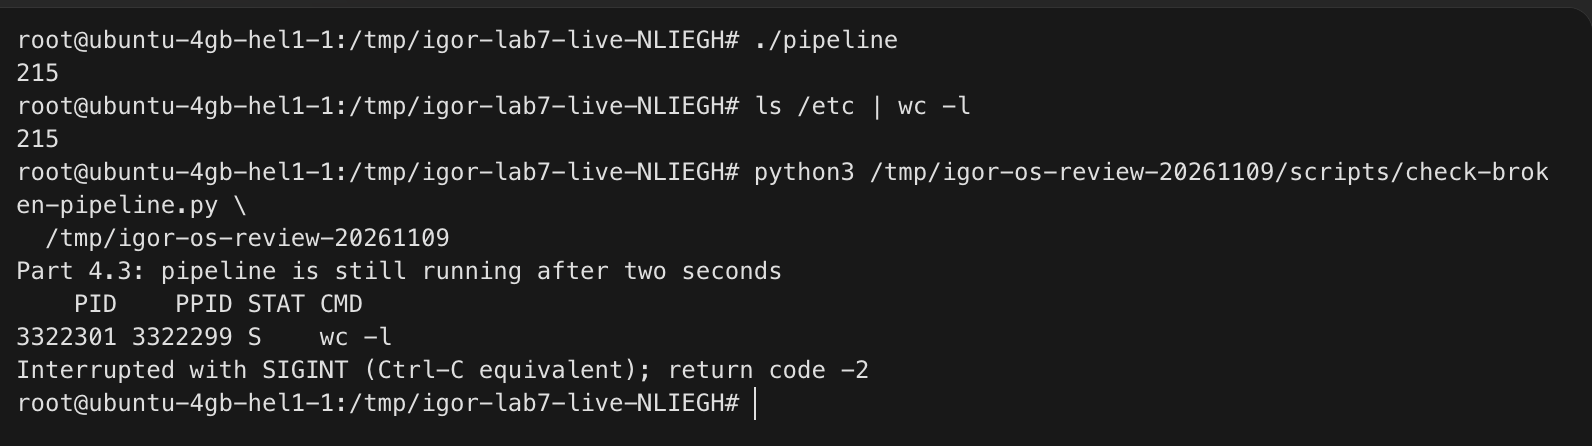
\includegraphics[width=\linewidth,height=0.67\textheight,keepaspectratio]{Lab7-8/evidence/screenshots/lab7-pipeline-terminal.png}
\end{minipage}\par\medskip

\par

\medskip\noindent

\begin{minipage}{\linewidth}\setstretch{1.0}
\captionof*{figure}{Figura 5. Native Terminal: live xv6 process replacement, failure status and two-pipe exchange}
\centering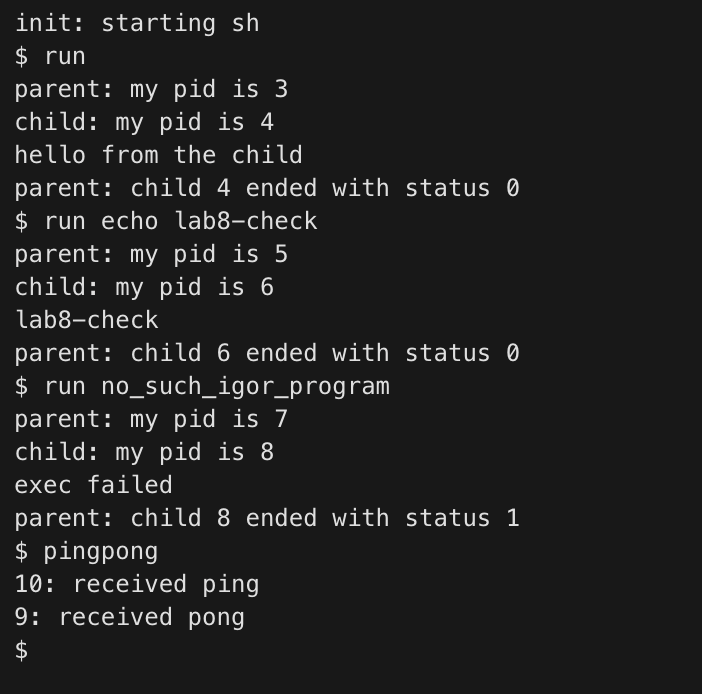
\includegraphics[width=\linewidth,height=0.67\textheight,keepaspectratio]{Lab7-8/evidence/screenshots/lab8-execution-terminal.png}
\end{minipage}\par\medskip

\subsection{Lab 8 source excerpts}\label{lab-8-source-excerpts}

The complete source is included under xv6/user. These listings are the
actual compiled program sources.

\begin{lstlisting}[language=C]
#include "kernel/types.h"
#include "user/user.h"

int
main(int argc, char *argv[])
{
  printf("parent: my pid is %d\n", getpid());
  int pid = fork();
  if(pid < 0){
    printf("fork failed\n");
    exit(1);
  }
  if(pid == 0){
    printf("child: my pid is %d\n", getpid());
    if(argc > 1){
      exec(argv[1], &argv[1]);
    } else {
      char *args[] = { "echo", "hello", "from", "the", "child", 0 };
      exec("echo", args);
    }
    printf("exec failed\n");
    exit(1);
  }
  int status;
  wait(&status);
  printf("parent: child %d ended with status %d\n", pid, status);
  exit(0);
}
\end{lstlisting}

\begin{lstlisting}[language=C]
#include "kernel/types.h"
#include "user/user.h"

int
main(void)
{
  int p2c[2], c2p[2];
  char b = 'x';
  if(pipe(p2c) < 0 || pipe(c2p) < 0){
    printf("pipe failed\n");
    exit(1);
  }
  int pid = fork();
  if(pid < 0){
    printf("fork failed\n");
    exit(1);
  }
  if(pid == 0){
    close(p2c[1]);
    close(c2p[0]);
    if(read(p2c[0], &b, 1) != 1) exit(1);
    printf("%d: received ping\n", getpid());
    if(write(c2p[1], &b, 1) != 1) exit(1);
    close(p2c[0]);
    close(c2p[1]);
    exit(0);
  }
  close(p2c[0]);
  close(c2p[1]);
  if(write(p2c[1], &b, 1) != 1) exit(1);
  if(read(c2p[0], &b, 1) != 1) exit(1);
  printf("%d: received pong\n", getpid());
  close(p2c[1]);
  close(c2p[0]);
  wait(0);
  exit(0);
}
\end{lstlisting}

\subsection{Lab 7 source excerpts}\label{lab-7-source-excerpts}

\subsubsection{run.c}\label{run.c}

\begin{lstlisting}[language=C]
    }
    if (pid == 0) {
        printf("child: my PID is %d, my parent is %d\n", getpid(), getppid());
        fflush(stdout);
        if (argc > 1)
            execvp(program, &argv[1]);
        else
            execlp("ls", "ls", "-l", (char *)NULL);
        perror("exec");
        _exit(127);
    }

    int status;
    if (waitpid(pid, &status, 0) < 0) {
        perror("waitpid");
        return 1;
    }
    if (WIFEXITED(status))
        printf("parent: child %d ended with status %d\n", pid, WEXITSTATUS(status));
    else if (WIFSIGNALED(status))
        printf("parent: child %d ended by signal %d\n", pid, WTERMSIG(status));
    return 0;
}
\end{lstlisting}

\subsubsection{zombie.c}\label{zombie.c}

\par\noindent\begin{minipage}{\linewidth}

\begin{lstlisting}[language=C]
    }
    if (pid == 0) {
        printf("child: my PID is %d, my parent is %d\n", getpid(), getppid());
        fflush(stdout);
        execlp("ls", "ls", "-l", (char *)NULL);
        perror("exec");
        _exit(127);
    }

    sleep(20);
    int status;
    if (waitpid(pid, &status, 0) < 0) {
        perror("waitpid");
        return 1;
    }
    if (WIFEXITED(status))
        printf("parent: child %d ended with status %d\n", pid, WEXITSTATUS(status));
    return 0;
\end{lstlisting}

\end{minipage}\par

\subsubsection{redirect.c}\label{redirect.c}

\par\noindent\begin{minipage}{\linewidth}

\begin{lstlisting}[language=C]
        close(STDOUT_FILENO);
        int fd = open("out.txt", O_WRONLY | O_CREAT | O_TRUNC, 0644);
        if (fd < 0) {
            perror("open");
            _exit(1);
        }
        fprintf(stderr, "open gave descriptor %d\n", fd);
        execlp("ls", "ls", "-l", (char *)NULL);
        perror("exec");
        _exit(127);
    }

    int status;
    if (waitpid(pid, &status, 0) < 0) {
        perror("waitpid");
        return 1;
    }
\end{lstlisting}

\end{minipage}\par

\subsubsection{pipeline.c}\label{pipeline.c}

\begin{lstlisting}[language=C]
        close(STDOUT_FILENO);
        if (dup(p[1]) != STDOUT_FILENO) _exit(1);
        close(p[0]);
        close(p[1]);
        execlp("ls", "ls", "/etc", (char *)NULL);
        perror("exec ls");
        _exit(127);
    }

    pid_t wc_pid = fork();
    if (wc_pid < 0) {
        perror("fork");
        close(p[0]);
        close(p[1]);
        waitpid(ls_pid, NULL, 0);
        return 1;
    }
    if (wc_pid == 0) {
        close(STDIN_FILENO);
        if (dup(p[0]) != STDIN_FILENO) _exit(1);
        close(p[0]);
        close(p[1]);
        execlp("wc", "wc", "-l", (char *)NULL);
        perror("exec wc");
        _exit(127);
    }

    close(p[0]);
    if (delay_eof) {
        fprintf(stderr, "parent keeps the write end open for 3 seconds; wc waits for EOF\n");
        sleep(3);
\end{lstlisting}

\par\noindent\begin{minipage}{\linewidth}

\section{Concluzie}\label{concluzie}

Experimentele explică execuția și comunicarea prin starea proceselor și
a descriptorilor. Colectarea copilului și închiderea corectă a capetelor
de pipe sunt necesare atât pentru rezultate corecte, cât și pentru
terminarea programelor.

\end{minipage}\par

\end{document}
